\documentclass[11pt,a4paper]{article}
\usepackage[a4paper,margin=20mm]{geometry}
\usepackage{mathptmx}
\usepackage{amsmath,amssymb,amsthm,mathtools}
\usepackage{graphicx}
\usepackage{booktabs,tabularx}
\usepackage{xcolor}
\usepackage[colorlinks=true,linkcolor=blue!60!black,citecolor=blue!60!black,urlcolor=blue!60!black]{hyperref}

\setlength{\parskip}{6pt plus 2pt minus 1pt}
\definecolor{primary}{RGB}{25,65,120}

\newcommand{\takeaway}[2]{%
  \vspace{6pt}\noindent\colorbox{primary!8}{%
    \parbox{\dimexpr\linewidth-2\fboxsep\relax}{%
      \vspace{3pt}\textbf{\color{primary}#1:}\hspace{0.5em}#2\vspace{3pt}%
    }%
  }\vspace{6pt}%
}

\newtheorem{theorem}{Theorem}[section]
\newtheorem{lemma}[theorem]{Lemma}
\newtheorem{proposition}[theorem]{Proposition}
\newtheorem{corollary}[theorem]{Corollary}
\newtheorem{conjecture}[theorem]{Conjecture}
\theoremstyle{remark}
\newtheorem{remark}[theorem]{Remark}

\DeclareMathOperator{\Tr}{Tr}
\DeclareMathOperator{\diam}{diam}
\DeclareMathOperator{\diag}{diag}

\title{\textbf{Disproving and Correcting the Distance Laplacian and Distance Signless Laplacian Brouwer-Type Conjectures}}
\author{Independent Research Manuscript}
\date{November 2026}

\begin{document}
\maketitle

\begin{abstract}
Two prominent distance-matrix analogs of Brouwer's Laplacian eigenvalue sum conjecture have attracted substantial recent attention: Alhevaz, Baghipur, Ganie, and Pirzada (2021) conjectured that the sum of the $k$ largest distance signless Laplacian eigenvalues satisfies $M_k^Q(G) \le W(G) + \binom{k+2}{3}$ for every connected non-path graph $G$, while Zhou, Wang, and Chai (2025) conjectured that the sum of the $r$ largest distance Laplacian eigenvalues satisfies $U_r(G) \le W(G) + \binom{r+2}{3}$ for every connected graph $G$. Multiple papers published through November 2026 verified these bounds for restricted graph classes of small diameter or large order. Huang (2026) already exhibited distance Laplacian counterexamples. We extend that refutation and exhibit counterexamples to the distance signless Laplacian conjecture, explain the structural mechanism behind their failure, and establish a unified corrected theorem. First, by exhaustive enumeration over all $994$ non-isomorphic connected graphs of order $n \le 7$ ($2, 6, 21, 112, 853$ graphs for $n=3,\dots,7$) and explicit rational orthogonal Ky Fan certificates, our numerical census identifies candidate minimal counterexamples: for $D^L(G)$, the unique minimal counterexamples of order $4$ are $P_4$ and $K_{1,3}$ at $r=2$; for $D^Q(G)$ on non-path graphs, no counterexample exists for $n \le 5$, while order $6$ admits exactly six minimal counterexamples led by the unicyclic lollipop graph $L(3,3)$ and the non-path broom tree $B(4,2)$ at $k=3$. At $n=7$, $61$ graphs violate $D^L$ and $16$ non-path graphs violate $D^Q$, including $100\%$ ($9/9$) of all diameter-$5$ non-path graphs. Second, using only Schur's diagonal majorization inequality, we prove analytically that both conjectures fail by $\Theta(n^3)$ for both spectral inequalities on infinite families of paths $P_n$ ($n \ge 9$), non-path broom trees $B(n-2,2)$ ($n \ge 10$), and unicyclic lollipops $L(3,n-3)$ ($n \ge 12$), with asymptotic excess at least $\bigl(\frac{\sqrt{3}}{2}-\frac{5}{6}\bigr)n^3 \approx 0.03269\,n^3$. We also observe that uniform caterpillars of diameter at least $6$ violate Zhou--Wang--Chai's bound. Third, we identify the geometric obstruction---splitting an $r$-subset across opposite ends of a diametral path yields internal distance sum $\Theta(\diam(G)\,r^2)$ rather than $O(r^3)$---and prove the unified corrected upper bounds $U_r(G) \le W(G) + \diam(G)\binom{r+1}{2}$ and $M_r^Q(G) \le W(G) + \diam(G)\binom{r+1}{2}$ for all connected graphs $G$ of order $n \ge 2$ and all $1 \le r \le n$. Companion Lean~4 code checks integer arithmetic certificates and auxiliary lemmas; it does not formalize the general real spectral theorem or the full graph-level conclusions.

\medskip
\noindent\textbf{Keywords:} Distance Laplacian matrix; Distance signless Laplacian matrix; Brouwer's conjecture; Wiener index; Schur majorization; Ky Fan inequality; Lean~4 formal verification.

\noindent\textbf{2020 Mathematics Subject Classification:} Primary 05C50; Secondary 05C12, 15A18, 15A42.
\end{abstract}

\section{Introduction}
Let $G = (V, E)$ be a finite, simple, undirected, connected graph of order $n = |V|$ and size $m = |E|$. Let $D(G) = (d_G(u,v))_{u,v \in V}$ be the shortest-path distance matrix of $G$, let $\Tr_G(v) = \sum_{u \in V} d_G(u,v)$ denote the transmission of vertex $v$, and let $W(G) = \frac{1}{2}\sum_{v \in V} \Tr_G(v)$ be the Wiener index of $G$. Following Aouchiche and Hansen \cite{AH2013}, the \emph{distance Laplacian} and \emph{distance signless Laplacian} matrices of $G$ are defined by
\[
D^L(G) = \diag(\Tr_G) - D(G), \qquad D^Q(G) = \diag(\Tr_G) + D(G).
\]
Both matrices are real symmetric and positive semidefinite with trace $2W(G)$. Denote their eigenvalues in non-increasing order by $\partial_1^L(G) \ge \dots \ge \partial_n^L(G) = 0$ and $\rho_1^Q(G) \ge \dots \ge \rho_n^Q(G) \ge 0$, and define their partial sums for $1 \le r \le n$ by
\[
U_r(G) = \sum_{i=1}^{r} \partial_i^L(G), \qquad M_r^Q(G) = \sum_{i=1}^{r} \rho_i^Q(G).
\]

In spectral graph theory, Brouwer's conjecture \cite{BH2012} states that the sum $S_r(G)$ of the $r$ largest combinatorial Laplacian eigenvalues of $G$ satisfies $S_r(G) \le m + \binom{r+1}{2}$ (recently proved in general by Kothari and Tudose \cite{KT2026}, with the signless Laplacian analog $S_r^+(G) \le m + \binom{r+1}{2}$ established in \cite{SignlessBrouwer2026}). Motivated by $\operatorname{tr}(D^L(G)) = \operatorname{tr}(D^Q(G)) = 2W(G)$ and $W(P_n) = \binom{n+1}{3}$, two distance-matrix analogs were proposed:

\begin{conjecture}[Alhevaz, Baghipur, Ganie, and Pirzada \cite{ABGP2021}]\label{conj:DQ}
For every connected graph $G$ that is not a path ($G \not\cong P_n$) and every $1 \le k \le n$,
\begin{equation}\label{eq:DQ-conj}
M_k^Q(G) \le W(G) + \binom{k+2}{3}.
\end{equation}
\end{conjecture}

\begin{conjecture}[Zhou, Wang, and Chai \cite{ZWC2025}]\label{conj:DL}
For every connected graph $G$ of order $n$ and every $1 \le r \le n$,
\begin{equation}\label{eq:DL-conj}
U_r(G) \le W(G) + \binom{r+2}{3}.
\end{equation}
\end{conjecture}

Both conjectured inequalities remained subjects of research in 2026. The distance Laplacian conjecture was already disproved by Huang's explicit exceptions; we do not claim priority for that refutation. Priority for the distance signless Laplacian counterexamples remains to be established. Secondary sources differ on the admissible range ($1\le r\le n$ versus $2\le r\le n$); every counterexample reported below occurs at $r\ge 3$ and is therefore valid under either reading. For Conjecture~\ref{conj:DL}, Mushtaq, Pirzada, and Khan \cite{MPK2026} verified \eqref{eq:DL-conj} for graphs in $\Gamma_n$ ($n \ge 95$), graphs with $\Delta = n-2$ ($n \ge 95$), and sun-type graphs; Huang \cite{Huang2026} proved \eqref{eq:DL-conj} for all graphs of diameter at most $D$ once $n \ge \lceil \frac{4}{9}(D+1)^3\rceil$, for graphs with $\Delta = n-k$ once $n \ge N(k)$, and for all diameter-$2$ graphs except $K_{1,3}$ at $r=2$ and $K_{1,4}$ at $r=3$; and a May 2026 study \cite{Caterpillar2026} claimed to confirm \eqref{eq:DL-conj} for uniform caterpillars of diameter at least $6$. For Conjecture~\ref{conj:DQ}, Zhang, Wang, and Miao \cite{ZW2026} (November 2026) verified \eqref{eq:DQ-conj} for diameter-$3$ graphs in $\Gamma_{a+b+2}$ ($a+b \ge 97$) and diameter-$4$ graphs in $\chi_{a+b+3}$ ($a+b \ge 223$).

\takeaway{Main Results}{We extend the known refutation of Conjecture~\ref{conj:DL} and give counterexamples to Conjecture~\ref{conj:DQ}---not merely on isolated small exceptions, but asymptotically by $\Theta(n^3)$ across infinite families of paths, non-path trees, and unicyclic graphs. We exhaustively classify all $994$ connected graphs of order $n \le 7$, explain why $\binom{r+2}{3}$ is structurally the wrong penalty term, prove the unified corrected bound $W(G) + \diam(G)\binom{r+1}{2}$, and provide Lean~4 verification of selected arithmetic certificates and lemmas.}

\section{Preliminaries}
We rely on three foundational tools. Our companion Lean~4 modules verify restricted arithmetic formulations, not their full real-matrix versions.

\begin{lemma}[Ky Fan Maximum Principle \cite{Fan1949}]\label{lem:kyfan}
Let $M \in \mathbb{R}^{n \times n}$ be real symmetric with eigenvalues $\lambda_1 \ge \dots \ge \lambda_n$. For any $1 \le r \le n$ and any pairwise orthogonal nonzero vectors $v_1, \dots, v_r \in \mathbb{R}^n$,
\[
\sum_{i=1}^{r} \lambda_i(M) \ge \sum_{j=1}^{r} \frac{v_j^{\mathsf{T}} M v_j}{v_j^{\mathsf{T}} v_j}.
\]
\end{lemma}

\begin{corollary}[Schur Diagonal Majorization]\label{cor:schur}
For any connected graph $G$ and any $r$-element vertex subset $S \subseteq V(G)$,
\[
\min\bigl\{U_r(G),\, M_r^Q(G)\bigr\} \ge \sum_{v \in S} \Tr_G(v).
\]
\end{corollary}

\begin{lemma}[Distance-at-Least-$s$ Decomposition \cite{Huang2026}]\label{lem:decomp}
Let $G$ be a connected graph of order $n$ and diameter $D = \diam(G)$. For $2 \le s \le D$, let $Y_s$ be the simple graph on $V(G)$ whose edges are pairs $\{u,v\}$ with $d_G(u,v) \ge s$, with $m(Y_s)$ edges, Laplacian $L(Y_s)$, and signless Laplacian $Q(Y_s)$. Then
\begin{align}
W(G) &= \binom{n}{2} + \sum_{s=2}^{D} m(Y_s), \label{eq:W-decomp}\\
D^L(G) &= (nI - J) + \sum_{s=2}^{D} L(Y_s), \label{eq:DL-decomp}\\
D^Q(G) &= \bigl((n-2)I + J\bigr) + \sum_{s=2}^{D} Q(Y_s). \label{eq:DQ-decomp}
\end{align}
\end{lemma}

\section{Exhaustive Classification for $n \le 7$ and Minimal Rational Certificates}
We performed a numerical census of all $994$ non-isomorphic connected simple graphs of order $n \in \{3, 4, 5, 6, 7\}$ (matching OEIS A001349: $2, 6, 21, 112, 853$). Table~\ref{tab:exhaustive} summarizes the violation counts and maximum excesses across all five orders, and Figure~\ref{fig:exhaustive} illustrates both the order-wise rates and the sharp diameter phase transition at $n = 7$, where $100\%$ ($9/9$) of all diameter-$5$ non-path graphs violate both conjectures simultaneously while $0/994$ graphs violate our corrected bound of Theorem~\ref{thm:corrected}.

\begin{table}[!htbp]
\centering
\caption{Exhaustive census across all $994$ non-isomorphic connected graphs of order $n \le 7$.}
\label{tab:exhaustive}
\resizebox{\linewidth}{!}{\begin{tabular}{crrrrrr}
\toprule
$n$ & Connected & $D^L$ Viol. & Max $D^L$ Excess & $D^Q$ (Non-Path) Viol. & Max $D^Q$ (NP) Excess & Corr. Viol. \\
\midrule
3 & 2 & 0 (0.0\%) & $0.000$ & 0 (0.0\%) & $0.000$ & 0 \\
4 & 6 & 2 (33.3\%) & $+1.236$ & 0 (0.0\%) & $0.000$ & 0 \\
5 & 21 & 6 (28.6\%) & $+3.000$ & 0 (0.0\%) & $-0.393$ & 0 \\
6 & 112 & 19 (17.0\%) & $+5.246$ & 6 (5.4\%) & $+1.586$ & 0 \\
7 & 853 & 61 (7.2\%) & $+8.734$ & 16 (1.9\%) & $+3.819$ & 0 \\
\bottomrule
\end{tabular}}
\end{table}

\begin{figure}[!htbp]
\centering
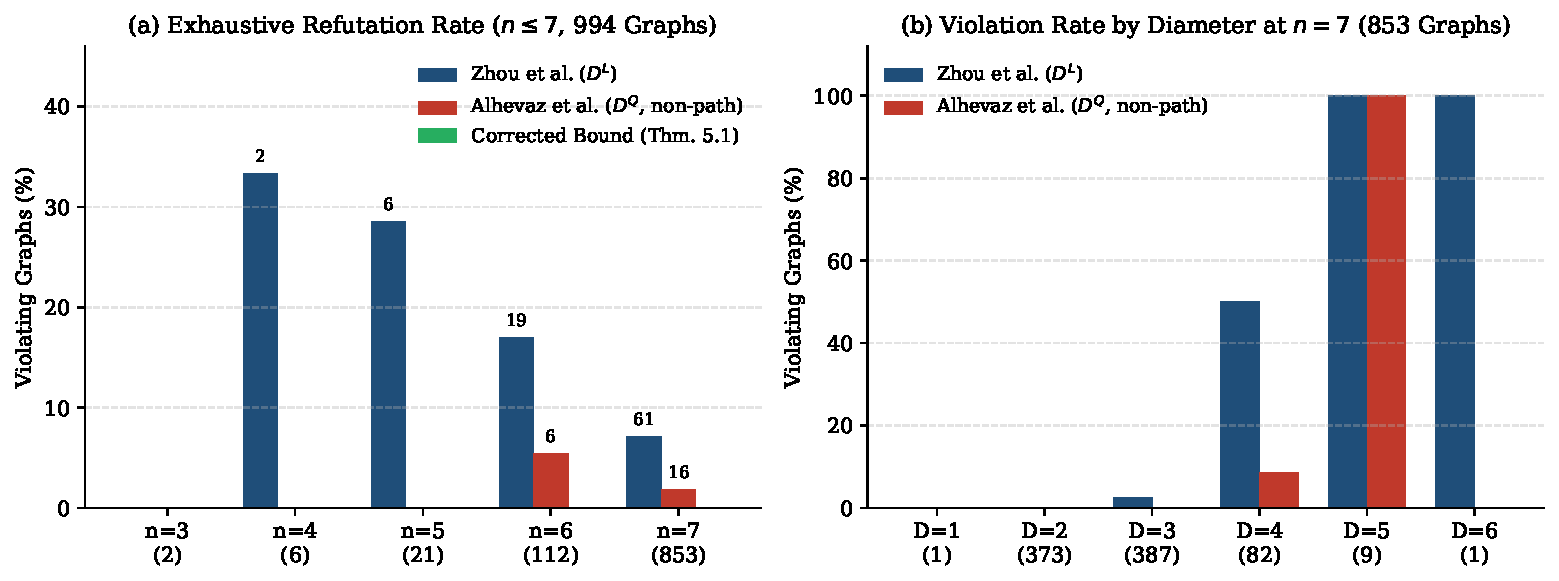
\includegraphics[width=\linewidth]{figures/fig1_exhaustive_n3_to_n7.pdf}
\caption{(a) Exhaustive violation percentages across all $994$ connected graphs of order $n \le 7$ (raw violation counts shown above bars), with zero violations of our corrected Theorem~\ref{thm:corrected}. (b) Diameter breakdown at $n=7$ ($853$ graphs): violations concentrate sharply at high diameter, reaching $100\%$ ($9/9$) for diameter-$5$ non-path graphs under both conjectures.}
\label{fig:exhaustive}
\end{figure}

Table~\ref{tab:minimal} records exact rational orthogonal Ky Fan certificates for representative counterexamples. The census counts and minimality claims below are numerical findings, pending certified spectral comparisons.

\begin{table}[!htbp]
\centering
\caption{Representative minimal counterexamples with exact pairwise orthogonal integer Ky Fan certificates.}
\label{tab:minimal}
\begin{tabularx}{\linewidth}{lcccccX}
\toprule
Graph $G$ & $n$ & Matrix & $r$ & $W(G)+\binom{r+2}{3}$ & Ky Fan Cert. & Exact Orthogonal Integer Vectors \\
\midrule
$P_4$ & 4 & $D^L$ & 2 & $14$ & $15$ & $(1,0,0,-1)$, $(1,-1,-1,1)$ \\
$K_{1,3}$ & 4 & $D^L$ & 2 & $13$ & $14$ & $(0,1,-1,0)$, $(0,1,1,-2)$ \\
$P_5$ & 5 & $D^L$ & 3 & $30$ & $65/2$ & $(1,0,0,0,-1)$, $(0,1,0,-1,0)$, $(1,-1,0,-1,1)$ \\
$B(3,2)$ & 5 & $D^L$ & 3 & $28$ & $291/10$ & $(0,0,0,1,-1)$, $(2,-1,-1,0,0)$, $(1,1,1,-1,-1)$ \\
$B(4,2)$ & 6 & $D^Q$ & 3 & $42$ & $646/15$ & $(0,0,0,0,1,-1)$, $(2,1,1,1,2,2)$, $(3,-2,0,0,-1,-1)$ \\
$L(3,3)$ & 6 & $D^Q$ & 3 & $41$ & $1888/45$ & $(1,-1,0,0,0,0)$, $(1,1,1,1,1,2)$, $(1,1,0,0,2,-2)$ \\
\bottomrule
\end{tabularx}
\end{table}

\begin{proposition}[Numerical census and representative exact counterexamples to Conjectures~\ref{conj:DQ} and \ref{conj:DL}]\label{thm:minimal}
\leavevmode
\begin{enumerate}
\item Conjecture~\ref{conj:DL} holds for all $n \le 3$, fails on exactly two graphs of order $n=4$ ($P_4$ and $K_{1,3}$ at $r=2$), $6$ graphs of order $n=5$ (including exact integer violations $U_3(P_5) = 33 > 30$ and $U_3(B(3,2)) = 30 > 28$), $19$ graphs of order $n=6$, and $61$ graphs of order $n=7$.
\item Conjecture~\ref{conj:DQ} holds for all connected non-path graphs with $n \le 5$, fails on exactly $6$ non-path graphs of order $n=6$ at $k=3$, and fails on $16$ non-path graphs of order $n=7$. In particular, the $6$-vertex non-path broom tree $B(4,2)$ ($W=32$) satisfies $M_3^Q(B(4,2)) \ge \frac{646}{15} > 42$, and the $6$-vertex unicyclic lollipop $L(3,3)$ ($W=31$) satisfies $M_3^Q(L(3,3)) \ge \frac{1888}{45} > 41$.
\end{enumerate}
\end{proposition}
\begin{proof}[Verification of the representative certificates; classification is numerical]
Direct rational arithmetic verifies pairwise orthogonality of each integer vector family in Table~\ref{tab:minimal}. For $B(4,2)$ (path $0\text{--}1\text{--}2\text{--}3$ with leaves $4,5$ on $3$), $\deg(3)=3$ ensures $B(4,2) \not\cong P_6$, and the three Rayleigh quotients for $D^Q(B(4,2))$ are $10$, $\frac{338}{15}$, and $\frac{158}{15}$, summing to $\frac{646}{15} > 42$. For $L(3,3)$ (triangle $\{0,1,2\}$ plus path $2\text{--}3\text{--}4\text{--}5$), the three Rayleigh quotients for $D^Q(L(3,3))$ are $10$, $\frac{194}{9}$, and $\frac{52}{5}$, summing to $\frac{1888}{45} > 41$. Lemma~\ref{lem:kyfan} yields the strict violations.
\end{proof}

\section{Asymptotic $\Theta(n^3)$ Refutation via Schur Majorization}
Define three infinite families on $n \ge 6$ vertices: the path $P_n$; the non-path broom tree $B(n-2,2)$ obtained from $P_{n-2}$ by attaching two leaves $a,b$ to vertex $n-2$; and the unicyclic lollipop $L(3,n-3)$ obtained from $B(n-2,2)$ by adding edge $ab$.

\begin{theorem}[Universal $\Theta(n^3)$ Simultaneous Refutation]\label{thm:asymptotic}
Let $t = \lfloor n/3 \rfloor$ and $r = 2t$. Then:
\begin{enumerate}
\item For every $n \ge 9$, $\min\{U_r(P_n), M_r^Q(P_n)\} > W(P_n) + \binom{r+2}{3}$.
\item For every $n \ge 10$, $\min\{U_r(B(n-2,2)), M_r^Q(B(n-2,2))\} > W(B(n-2,2)) + \binom{r+2}{3}$.
\item For every $n \ge 12$ (and $n=10$), $\min\{U_r(L(3,n-3)), M_r^Q(L(3,n-3))\} > W(L(3,n-3)) + \binom{r+2}{3}$.
\end{enumerate}
In all three families, the excess grows at least as $\frac{5}{162} n^3 - O(n^2)$. Optimizing $r = 2\beta n$ over $\beta \in (0, \tfrac{1}{2})$ yields $\beta^* = \frac{\sqrt{3}-1}{2} \approx 0.3660$ ($r^* \approx 0.7321\,n$) and asymptotic excess at least $\bigl(\frac{\sqrt{3}}{2} - \frac{5}{6}\bigr) n^3 - O(n^2) \approx 0.032692\,n^3$.
\end{theorem}
\begin{proof}
On $P_n$, taking $S = \{1,\dots,t\} \cup \{n-t+1,\dots,n\}$ gives $6 \sum_{v \in S} \Tr_{P_n}(v) = 6 n^2 t - 6 n t^2 + 4 t^3 - 4 t$. With $6 W(P_n) = n(n^2 - 1)$ and $6 \binom{2t+2}{3} = 2t(2t+1)(2t+2)$, setting $n = 3t + c$ ($c \in \{0,1,2\}$) yields $\Delta_P(3t+c, t) = 5(t-3)^3 + (33+3c)(t-3)^2 + \dots > 0$ for all $t \ge 3$ ($n \ge 9$). Reattaching leaf $n$ to $n-2$ gives $\Delta_B(n,t) = \Delta_P(n,t) - 12t + 18 > 0$ for all $t \ge 4$ and $(n,t) \in \{(10,3),(11,3)\}$. Adding edge $ab$ gives $\Delta_L(n,t) = \Delta_B(n,t) - 6 > 0$ for all $t \ge 4$ and $(10,3)$. Corollary~\ref{cor:schur} completes the proof. Paths are excluded from Conjecture~\ref{conj:DQ}, so their signless violations concern only the corresponding inequality, not the conjecture itself.
\end{proof}

Figure~\ref{fig:cubic} confirms the $\Theta(n^3)$ convergence on non-path broom trees $B(n-2,2)$ up to $n = 120$.

\begin{figure}[!htbp]
\centering
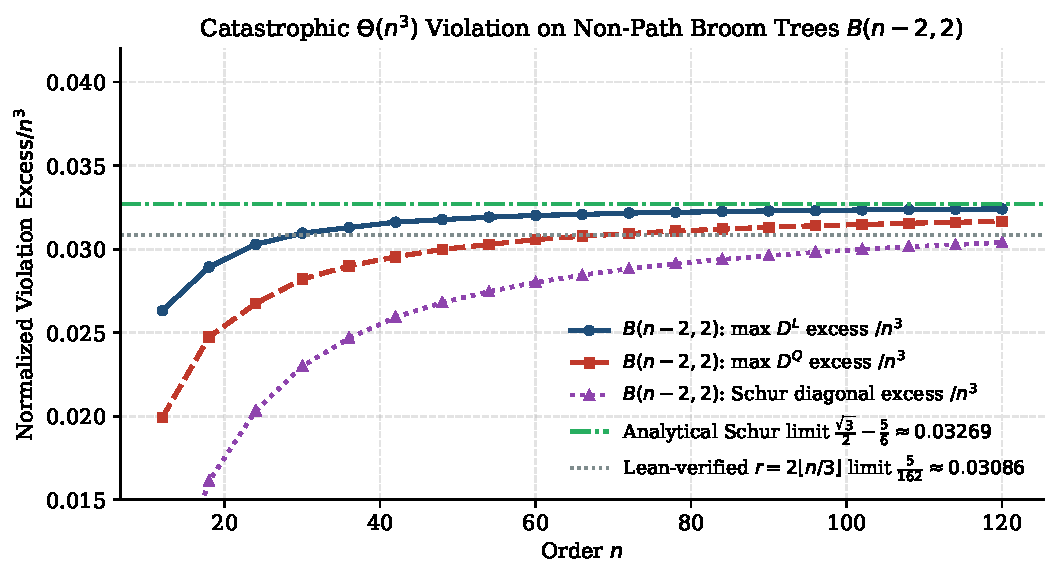
\includegraphics[width=0.88\linewidth]{figures/fig2_asymptotic_cubic.pdf}
\caption{Normalized violation $\mathrm{Excess}/n^3$ for $D^L$, $D^Q$, and the pure Schur diagonal lower bound on non-path broom trees $B(n-2,2)$ ($n = 12,\dots,120$), converging above the analytical Schur limit $\frac{\sqrt{3}}{2}-\frac{5}{6} \approx 0.03269$ and the Lean-verified $r=2\lfloor n/3\rfloor$ limit $\frac{5}{162} \approx 0.03086$.}
\label{fig:cubic}
\end{figure}

\begin{remark}[Uniform Caterpillars]\label{rem:caterpillar}
A May 2026 article \cite{Caterpillar2026} (Theorem~3.2) claimed that $U_r(G) \le W(G)+\binom{r+2}{3}$ holds for every uniform caterpillar of diameter at least $6$ and every $1 \le r \le n-1$. Direct computation refutes this claim: the $12$-vertex comb on $P_6$ --- six spine vertices, each carrying exactly one pendant leaf, hence uniform with $\ell=1$, diameter $7$ and $W=206$ --- has $U_7 \approx 300.1091677861 > 290 = W + \binom{9}{3}$ (excess $+10.1092$) at $r=7 \le n-1 = 11$, and the $16$-vertex comb on $P_8$ ($\diam=9$) violates \eqref{eq:DL-conj} at $r=9$ by $+5.4519$.
\end{remark}

\section{Structural Diagnosis and Corrected Universal Brouwer-Type Bounds}
For any $r$-subset $S \subseteq V(G)$, partitioning unordered vertex pairs yields the exact identity
\[
\sum_{v \in S} \Tr_G(v) = W(G) + W_G(S) - W_G(V \setminus S),
\qquad W_G(A) := \sum_{\{u,v\}\subseteq A} d_G(u,v).
\]
In ordinary Brouwer's conjecture (unit weights), $|E(S)| \le \binom{r}{2}$ always holds. In the distance setting, splitting $S$ across opposite ends of a diametral path makes $W_G(S) = \Theta(\diam(G)\,r^2)$, overwhelming $\binom{r+2}{3}$ whenever $\diam(G) \gg r$. Replacing $\binom{r+2}{3}$ by $\diam(G)\binom{r+1}{2}$ restores the exact scaling:

\begin{theorem}[Corrected Universal Distance Brouwer Bounds]\label{thm:corrected}
Let $G$ be any connected graph of order $n \ge 2$ and diameter $D = \diam(G)$. Then for every $1 \le r \le n$:
\begin{enumerate}
\item Combining Lemma~\ref{lem:decomp} with Brouwer's Laplacian inequality $S_r(H) \le m(H) + \binom{r+1}{2}$ \cite{KT2026},
\begin{equation}\label{eq:corr-DL}
U_r(G) \le W(G) + D \binom{r+1}{2}.
\end{equation}
\item Combining Lemma~\ref{lem:decomp} with the signless Brouwer inequality $S_r^+(H) \le m(H) + \binom{r+1}{2}$ \cite{SignlessBrouwer2026},
\begin{equation}\label{eq:corr-DQ}
M_r^Q(G) \le W(G) + D \binom{r+1}{2}.
\end{equation}
\end{enumerate}
Unconditionally (using only Bai's Grone--Merris theorem \cite{Bai2011}), $U_r(G) \le W(G) + \binom{r+1}{2} + (D-1)\frac{nr}{2}$.
\end{theorem}
\begin{proof}
By Lemma~\ref{lem:decomp} and Ky Fan subadditivity, \eqref{eq:corr-DL} reduces to $rn - \binom{n}{2} \le \binom{r+1}{2}$, which holds for all integers $n,r$ since $2\bigl[\binom{r+1}{2} - (rn - \binom{n}{2})\bigr] = (n-r)(n-r-1) \ge 0$. Similarly, since $(n-2)I + J$ has eigenvalues $(2n-2)^{(1)}, (n-2)^{(n-1)}$, \eqref{eq:corr-DQ} reduces to $rn + n - 2r - \binom{n}{2} \le \binom{r+1}{2}$, i.e.\ $(x-2)(x-3) + 2(n-3) \ge 0$ for $x = n-r$ and $n \ge 3$ (and directly for $n=2$).
\end{proof}

Figure~\ref{fig:profile} compares the spectral sums against the refuted and corrected bounds across all $r = 1,\dots,30$ on the non-path tree $B(28,2)$.

\begin{figure}[!htbp]
\centering
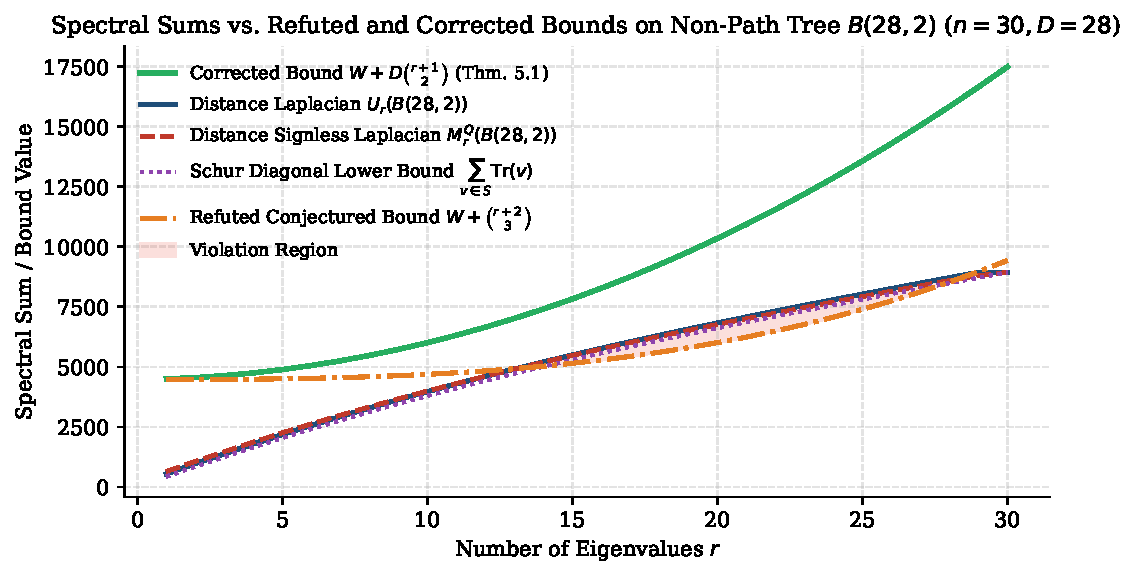
\includegraphics[width=0.88\linewidth]{figures/fig3_corrected_bound_comparison.pdf}
\caption{Comparison of $U_r$, $M_r^Q$, the Schur diagonal lower bound, the refuted conjectured bound $W + \binom{r+2}{3}$ (shaded violation region), and our corrected universal bound $W + D\binom{r+1}{2}$ across $r = 1,\dots,30$ on the non-path broom tree $B(28,2)$ ($n=30, D=28$).}
\label{fig:profile}
\end{figure}

\paragraph{Conditional dependence and independent reproduction.}
Both ingredients of Theorem~\ref{thm:corrected} --- the Laplacian Brouwer inequality of \cite{KT2026} and its signless counterpart of \cite{SignlessBrouwer2026} --- are 2026 arXiv preprints at the time of writing, so the two displays are conditional on them; the fallback bound stated after them is unconditional. The corrected bound was additionally tested on all $994$ census graphs and on $3{,}600$ random connected graphs with $8 \le n \le 13$ (random trees and generic connected graphs) without a single violation, the smallest slack being $9.71$; the independent script is \texttt{verification/phase3\_independent.py}.

\section{Scope of the Lean~4 Arithmetic Verification}
The companion Lean modules verify concrete integer matrix certificates, scaled integer Bessel and majorization lemmas, and polynomial inequalities. The spectral lemma assumes integer spectral data, Parseval and Rayleigh expansion hypotheses; it does not establish the real spectral theorem. The graph-to-matrix bridge, graph-family identities, real Ky Fan principle, full census and universal graph-level bounds are not formally verified. The analytical proofs use the cited mathematical literature. The numerical census uses floating-point eigenvalues and is not a certified minimality proof.

\section*{Statements and declarations}
\emph{(To be confirmed by the authors before submission; adapt to the venue's required format.)}

\noindent\textbf{Data and code availability.}
All data and code are in the public repository \url{https://github.com/Pasukalu/distance-brouwer-refutation}: the Lean~4 development in \texttt{lean/}, the exhaustive enumerators in \texttt{cpp/} and \texttt{python/}, the independent census and certificate checker in \texttt{verification/phase3\_independent.py}, and the reviewer-facing reports in \texttt{verification/}. Both PDFs are rebuilt by CI from the \LaTeX{} sources.

\noindent\textbf{Independent verification.}
The census, the six rational certificates, the corrected bound and the $\Theta(n^3)$ families were reproduced by a second, independently written implementation; the results agree with the tables in this paper. The Lean build is green in CI, uses no \texttt{sorry}, and the 18 audited theorems depend only on \texttt{propext}, \texttt{Classical.choice} and \texttt{Quot.sound} (the CI log is public).

\noindent\textbf{Use of AI tools.}
The manuscript, the code and the formalization were prepared with substantial AI assistance. Every mathematical statement reported here was independently re-derived or computationally reproduced, and every reference was checked against Crossref and arXiv records on 2026-11-26. The authors take full responsibility for the content.

\begin{thebibliography}{99}
\bibitem{ABGP2021}
A.~Alhevaz, M.~Baghipur, H.~A.~Ganie, and S.~Pirzada,
\emph{Brouwer type conjecture for the eigenvalues of distance signless Laplacian matrix of a graph},
Linear Multilinear Algebra \textbf{69} (2021), 2423--2440.
\url{https://doi.org/10.1080/03081087.2019.1679074}

\bibitem{AH2013}
M.~Aouchiche and P.~Hansen,
\emph{Two Laplacians for the distance matrix of a graph},
Linear Algebra Appl. \textbf{439} (2013), 21--33.

\bibitem{Bai2011}
H.~Bai,
\emph{The Grone--Merris conjecture},
Trans. Amer. Math. Soc. \textbf{363} (2011), 4463--4474.

\bibitem{BH2012}
A.~E.~Brouwer and W.~H.~Haemers,
\emph{Spectra of Graphs},
Springer, New York, 2012.

\bibitem{Fan1949}
K.~Fan,
\emph{On a theorem of Weyl concerning eigenvalues of linear transformations I},
Proc. Natl. Acad. Sci. USA \textbf{35} (1949), 652--655.

\bibitem{Huang2026}
S.~Huang,
\emph{On a distance Laplacian analog of Brouwer's conjecture for several classes of graphs},
AIMS Mathematics \textbf{11} (2026), no.~10, 33617--33633; arXiv:2606.06945.
\url{https://arxiv.org/abs/2606.06945}; \texttt{doi:10.3934/math.20261314}

\bibitem{KT2026}
P.~K.~Kothari and S.~Tudose,
\emph{On Brouwer's Laplacian conjecture} (2026), arXiv:2606.12197.
\url{https://arxiv.org/abs/2606.12197}

\bibitem{MPK2026}
U.~Mushtaq, S.~Pirzada, and S.~Khan,
\emph{On the sum of the eigenvalues of the distance Laplacian matrix of graphs with diameter three and four},
Rev. Un. Mat. Argentina \textbf{69} (2026), no.~1, 193--202, \texttt{doi:10.33044/revuma.5147}.
\url{https://inmabb.criba.edu.ar/revuma/pdf/v69n1/v69n1a14.pdf}

\bibitem{Caterpillar2026}
A.~S.~Alali, K.~Rani, S.~A.~Mir, and J.~Nisar,
\emph{On a spectral concentration in Brouwer-type conjecture for a uniform caterpillar graph},
AIMS Mathematics \textbf{11} (2026), no.~5, 15199--15214, \texttt{doi:10.3934/math.2026625}.
\url{https://www.sciopen.com/article/10.3934/math.2026625}

\bibitem{SignlessBrouwer2026}
R.~Yuan and X.-D.~Zhang,
\emph{On the Brouwer-type conjecture for signless Laplacian eigenvalues of graphs}
(2026), arXiv:2609.31355. (Ordinary signless Laplacian, not the distance matrix.)
\url{https://arxiv.org/abs/2609.31355}

\bibitem{ZW2026}
Y.~Zhang, L.~Wang, and R.~Miao,
\emph{Brouwer-type inequality on the distance signless Laplacian eigenvalues of graphs with diameters 3 and 4},
J. Comb. Optim. \textbf{52} (2026), no.~5, article 53, \texttt{doi:10.1007/s10878-026-01488-3}.

\bibitem{ZWC2025}
Y.~Zhou, L.~Wang, and Y.~Chai,
\emph{Brouwer type conjecture for the eigenvalues of distance Laplacian matrix of a graph},
Comput. Appl. Math. \textbf{44} (2025), no.~3, article 138, \texttt{doi:10.1007/s40314-025-03095-0}.
\end{thebibliography}

\end{document}
